\documentclass[10pt,twocolumn]{article}
\usepackage[a4paper,margin=1.65cm]{geometry}
\usepackage{amsmath,amssymb,booktabs,graphicx,microtype,url,array}
\usepackage[hidelinks]{hyperref}
\usepackage[numbers,sort&compress]{natbib}
\usepackage{tikz}
\usetikzlibrary{arrows.meta,positioning}
\graphicspath{{figures/}}
\setlength{\columnsep}{0.65cm}

\title{From Waveform Fidelity to Cardiac Representation:\\
Failure Mechanisms in Ballistocardiographic Heart-Rate Estimation}
\author{Joseph (Hao Hsiang) Wang\\
\small Independent Researcher\\
\small \texttt{josephwang2400@gmail.com}}
\date{}

\begin{document}
\maketitle

\begin{abstract}
Ballistocardiographic (BCG) heart-rate estimation is difficult because the measured mechanical waveform reflects cardiac activity only after transmission through the body, support surface, sensor coupling, respiration, and noise. This study asks which mechanical-signal representations preserve information useful to an interpretable downstream estimator, how those representations fail, and whether conventional waveform repair restores task fidelity. We evaluated a six-band rectification and harmonic-consistency estimator, HeartV6, on 9,006 synchronized ten-second BCG--ECG windows from repeated recordings of one individual. HeartV6 achieved 2.28 beats per minute (BPM) mean absolute error and 93.64\% within 5 BPM. A controlled amplitude-modulation experiment recovered known modulation in 94.14\% of full-wave-rectified cases versus 7.41\% from the raw spectrum, demonstrating a signal-processing mechanism without asserting a physiological generative model. Among 573 real-window errors above 5 BPM, representation weakness was the largest resolved category (37.35\%), followed by interval refinement (19.90\%) and isolated fusion/scoring failure (9.08\%); 33.68\% remained mixed or unresolved. Controlled noise, clipping, and sample loss jointly reduced target dominance and cross-band or harmonic-family consistency while increasing spectral entropy. Their dominant degradation direction explained 49.61\% of multifeature variation and resembled natural representation failure, most strongly for clipping (cosine similarity 0.924). Conventional filtering and interpolation did not reliably reverse these effects: severe-noise band-limiting improved error by only 0.05 BPM, while clipping and missing-sample interpolation worsened aggregate performance. Waveform reconstruction recovery was only weakly associated with heart-rate improvement ($\rho=0.067$). These results indicate that, for the evaluated pipeline and recordings, waveform similarity and downstream cardiac-information fidelity are distinct objectives, motivating future methods that preserve task-relevant spectral, cross-band, and harmonic structure.
\end{abstract}

\section{Introduction}
Ballistocardiography measures mechanical motion induced by cardiovascular activity and can be embedded in beds and other support surfaces for unobtrusive monitoring \cite{sadek2019review,qiu2025dataset}. The recorded waveform is not a direct cardiac source signal: body mechanics, posture, respiration, mattress dynamics, sensor coupling, and environmental disturbance all shape the observation. A large spectral component can therefore correspond to a mechanical resonance or cardiac harmonic rather than the cardiac fundamental.

Prior heart-rate methods include peak detection, autocorrelation, probabilistic fusion, and learned regression \cite{brueser2020autocorrelation,jung2021loadcells,jiao2021bilstm}. Many signal-restoration approaches, however, are evaluated by waveform error even when the downstream estimator relies on a narrower set of periodic and cross-band features. Whether generic waveform fidelity is aligned with cardiac-rate fidelity remains an important sensing question.

This work studies that alignment through an interpretable estimator and controlled analyses. Its contributions are: (1) a reproducible multi-band BCG estimator and audited ECG reference; (2) a controlled demonstration of how nonlinear envelope operations expose low-frequency periodicity; (3) a full-dataset decomposition of representation, scoring, and interval-refinement failures; (4) paired robustness analysis under noise, saturation, and missing samples; and (5) a comparison showing that conventional waveform repair does not reliably restore estimator-relevant representation. All human data are repeated measurements of one individual; the results characterize these recordings and do not estimate population performance.

\section{Background and Estimator}
\subsection{Dataset and acquisition provenance}
The dataset contains 9,006 synchronized ten-second BCG--ECG windows sampled at 100~Hz. All recordings are from one individual under repeated dates, configurations, distances, and sensing conditions. Filename tokens historically named \texttt{Subject\_1} through \texttt{Subject\_10} are legacy dataset identifiers, not distinct participants.

Acquisition provenance was reconstructed by exact array-content comparison. Every window was matched to its declared 1,000-sample interval in one of 1,501 continuous source files; each source contributed six non-overlapping windows. Continuous-source identity is therefore verified, but ancestry above the source-file level remains unknown. Analyses preserve clean/degraded pairing and summarize heterogeneity by verified source. Window counts are descriptive and are not treated as independent biological replicates.

BCG input is filtered from 0.5--25~Hz and standardized per window. The ECG reference uses a Pan--Tompkins-inspired sequence of band-pass filtering, differentiation, squaring, moving integration, refractory peak selection, and local R-peak refinement \cite{pan1985qrs}. The audit retained legacy estimates for traceability and identified systematic reference disagreement in one legacy dataset group.

\subsection{Multi-band cardiac representation}
For BCG signal $x(t)$, HeartV6 uses six overlapping mechanical bands
\begin{equation}
\mathcal{B}=\{[1,5],[2,6],[3,7],[4,8],[5,9],[6,10]\}\ \mathrm{Hz}.
\end{equation}
Each band output is full-wave rectified. The fused magnitude spectrum is
\begin{equation}
P(f)=\sum_{b\in\mathcal{B}}\left|\mathcal{F}\{|H_b\{x\}|\}(f)\right|.
\end{equation}
For candidate fundamental $f$, the implementation sums local fused-spectrum energy around valid harmonics $kf<3$~Hz. If $N_f$ harmonic terms are valid, the production base score is
\begin{equation}
S_{\mathrm{prod}}(f)=\frac{1}{N_f+1}
\sum_{k: kf<3\,\mathrm{Hz}}\ \sum_{|\nu-kf|\leq0.15}P(\nu).
\label{eq:score}
\end{equation}
The additional denominator term is important empirically and is examined rather than silently changed. After the base family is selected, a factor of 2.5 favors its fundamental when comparing family members. Two narrow band-pass stages isolate the selected component; positive peaks yield the final mean interval and BPM. Confidence combines the harmonic-score margin and interval regularity.

\begin{figure}[t]
\centering
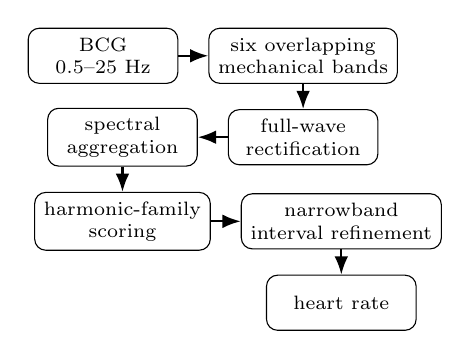
\begin{tikzpicture}[node distance=3.2mm and 3.8mm,>=Latex,
box/.style={draw,rounded corners,align=center,font=\scriptsize,minimum width=19mm,minimum height=7mm},arrow/.style={->,thick}]
\node[box] (x) {BCG\\$0.5$--$25$ Hz};
\node[box,right=of x] (bands) {six overlapping\\mechanical bands};
\node[box,below=of bands] (rect) {full-wave\\rectification};
\node[box,left=of rect] (fuse) {spectral\\aggregation};
\node[box,below=of fuse] (score) {harmonic-family\\scoring};
\node[box,right=of score] (time) {narrowband\\interval refinement};
\node[box,below=of time] (hr) {heart rate};
\draw[arrow] (x)--(bands); \draw[arrow] (bands)--(rect); \draw[arrow] (rect)--(fuse);
\draw[arrow] (fuse)--(score); \draw[arrow] (score)--(time); \draw[arrow] (time)--(hr);
\end{tikzpicture}
\caption{HeartV6 signal path. The study analyzes representation, fusion/scoring, and interval-refinement stages without changing production behavior.}
\label{fig:pipeline}
\end{figure}

\section{Experimental Methods}
\subsection{Controlled modulation analysis}
A synthetic signal tested whether nonlinear operations can expose known low-frequency modulation:
\begin{equation}
x(t)=[1+m\cos(2\pi f_m t)]\cos(2\pi f_c t)+\epsilon(t).
\end{equation}
Carrier frequencies were 4, 6, and 8~Hz; modulation frequencies were 0.8, 1.2, and 1.6~Hz; depths were 0.1, 0.3, and 0.6; and SNR was noise-free, 20, 10, or 0~dB. Three fixed-seed replicates produced 324 cases per method. Raw spectra, full-wave rectification, Hilbert envelopes, and squared energy were compared. Recovery required peak-frequency error no greater than 0.15~Hz. This is a controlled DSP experiment, not a physiological model of the real recordings.

\subsection{Failure-stage analysis}
Every real window was instrumented without modifying HeartV6. Recorded quantities included ECG reference, spectral and final HR, interval coefficient of variation (CV), peak count, score margin, target-to-distractor power ratio (T/D), spectral entropy, per-band preferred frequency, and cross-band agreement. Cross-band agreement is the fraction of six preferred frequencies lying within 0.15~Hz of their 0.1-Hz-binned mode.

Material failure was defined as final error above 5~BPM. Representation failure required mean T/D below 1 or ECG-target agreement in fewer than half the bands. Refinement failure required spectral error at most 3~BPM followed by more than 2~BPM worsening. Fusion/scoring failure required adequate representation, spectral error above 10~BPM, and a correct alternative from simple peak, term-normalized scoring, or modal per-band evidence. Overlapping or unsupported mechanisms remained mixed/unresolved.

The interval effect was
\begin{equation}
\Delta_{\mathrm{ref}}=|e_{\mathrm{final}}|-|e_{\mathrm{spectral}}|,
\end{equation}
where negative values indicate improvement. Current scoring was compared with fused-spectrum argmax and exact $1/N_f$ term normalization before interval refinement.

\subsection{Controlled sensing degradation}
Each preprocessed real BCG window was paired with Gaussian noise at 20, 10, and 0~dB; clipping at $\pm2$, $\pm1$, and $\pm0.5$ standard deviations; and deterministic contiguous zero-filled loss of 5, 15, and 30\%. Positive amplitude scaling by 0.75, 0.5, and 0.25 served as a negative control. Harmonic-family stability was the fraction of six per-band labels plus the fused label whose half/fundamental/double/other family matched clean. In total, 108,072 degraded pairs were evaluated.

\subsection{Conventional reconstruction baselines}
Fixed, non-tuned recovery methods were applied to clean/degraded pairs. Gaussian noise used a 0.5--12~Hz band-limit and five-point Wiener filter. Saturated samples were detected at the known clipping threshold and linearly interpolated while unaffected samples were retained. Missing samples used linear interpolation or shape-preserving piecewise cubic interpolation (PCHIP), with nearest-value boundary handling. Waveform recovery was
\begin{equation}
R_x=\frac{\mathrm{RMSE}(x_d,x_c)-\mathrm{RMSE}(x_r,x_c)}
{\mathrm{RMSE}(x_d,x_c)},
\end{equation}
for clean $x_c$, degraded $x_d$, and recovered $x_r$. Representation and HR changes were evaluated in paired form and summarized by continuous source.

\section{Results}
\subsection{Baseline heart-rate estimation}
Table~\ref{tab:baseline} gives descriptive performance on all 9,006 windows. HeartV6 reduced error relative to direct FFT and autocorrelation. These are within-person repeated-recording results, not estimates for unseen individuals.

\begin{table}[t]
\centering
\caption{Descriptive performance using the audited ECG reference.}
\label{tab:baseline}
\begin{tabular}{lrrrr}
\toprule
Method & MAE & RMSE & $\leq3$ & $\leq5$ \\
 & BPM & BPM & \% & \% \\
\midrule
FFT peak & 22.32 & 39.21 & 47.38 & 54.97 \\
Autocorrelation & 6.66 & 20.93 & 85.80 & 86.72 \\
HeartV6 & \textbf{2.28} & \textbf{7.15} & \textbf{88.13} & \textbf{93.64} \\
\bottomrule
\end{tabular}
\end{table}

The audited and legacy ECG estimates differed by 1.12~BPM on average, and 2.31\% differed by more than 5~BPM. In legacy group 7, reference correction reduced apparent HeartV6 MAE from 12.26 to 2.46~BPM, illustrating the importance of label audit before estimator optimization.

\subsection{Nonlinear exposure of modulation}
Full-wave rectification and Hilbert envelopes each recovered the known modulation in 94.14\% of 324 cases; squared energy recovered 94.44\%, while the raw spectrum recovered 7.41\%. Mean absolute frequency error was 0.032~Hz for rectification and Hilbert, 0.031~Hz for squared energy, and 1.115~Hz for raw spectra. All nonlinear methods achieved 100\% recovery through 10~dB and at 0~dB when modulation depth was at least 0.3. At 0~dB and depth 0.1, recovery fell to 29.6\% for rectification and Hilbert and 33.3\% for squared energy (Fig.~\ref{fig:am}).

\begin{figure*}[t]
\centering
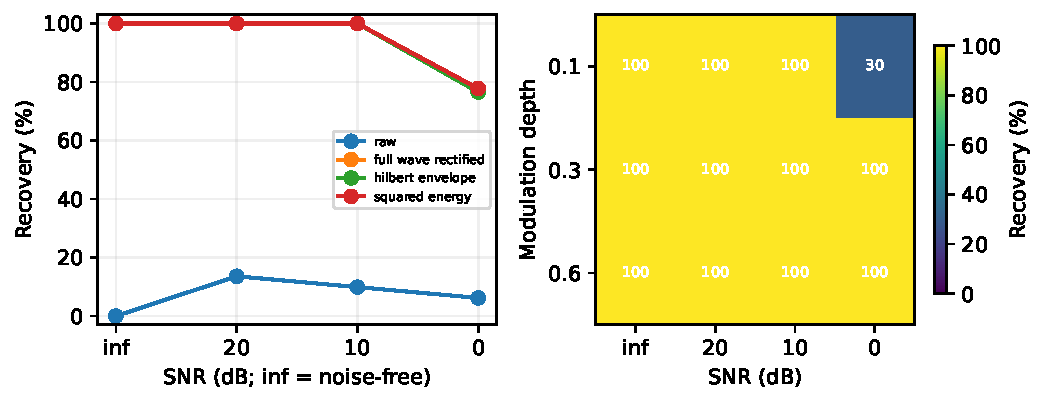
\includegraphics[width=0.96\textwidth]{am_mechanism.pdf}
\caption{Controlled amplitude-modulation analysis. Nonlinear envelope representations expose the known low-frequency component across most conditions (left); full-wave rectification fails mainly when modulation is shallow and SNR is 0~dB (right). The experiment demonstrates a DSP mechanism and does not establish a physiological BCG generative model.}
\label{fig:am}
\end{figure*}

\subsection{Failure mechanisms and interval refinement}
Of 9,006 windows, 8,433 were within 5~BPM and 573 were material failures. Among failures, representation weakness accounted for 214 (37.35\%), fusion/scoring for 52 (9.08\%), interval refinement for 114 (19.90\%), and mixed/unresolved mechanisms for 193 (33.68\%). Leaving ambiguous cases unresolved avoids overstating the taxonomy.

Spectral-only HR had 2.880~BPM MAE; interval refinement reduced this to 2.282~BPM. It improved 52.50\% of windows, worsened 19.88\%, and changed 27.63\% by at most 0.5~BPM. The strongest average benefit occurred for spectral errors of 3--10~BPM. For errors above 10~BPM, mean error changed from 37.998 to 38.085~BPM and 46.75\% worsened: interval timing cannot generally repair selection of the wrong frequency family (Fig.~\ref{fig:failure}).

\begin{figure*}[t]
\centering
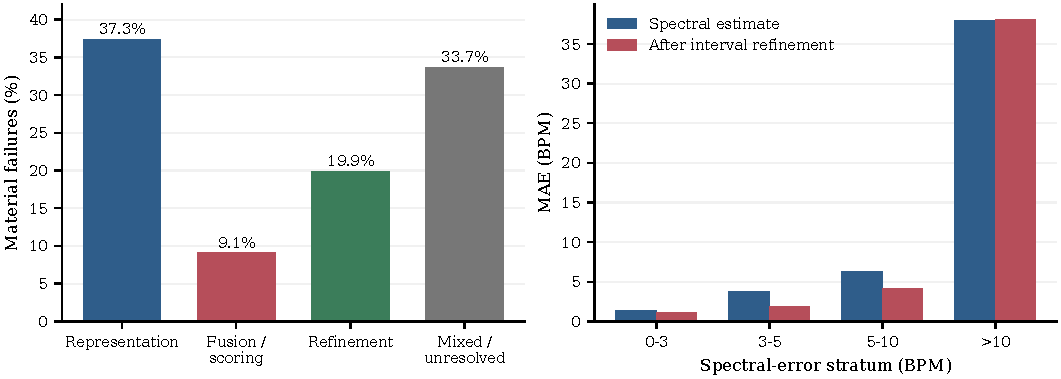
\includegraphics[width=0.94\textwidth]{failure_mechanisms.pdf}
\caption{Failure-stage analysis. Representation weakness was the largest resolved category among 573 material failures (left). Interval refinement substantially helped moderate spectral errors but did not repair gross family-selection errors (right).}
\label{fig:failure}
\end{figure*}

\subsection{Harmonic-scoring diagnostic}
The production score in Eq.~\ref{eq:score} implicitly favors candidates with more harmonic terms. Replacing it with exact $1/N_f$ normalization removed lower-boundary selections but increased double-rate errors from 0.46\% to 11.56\% and increased spectral MAE from 2.88 to 10.54~BPM. Simple argmax similarly produced 11.08\% double-rate errors and 9.63~BPM MAE. The production scorer selected the 0.7-Hz lower boundary in 0.80\% of windows and never selected the upper boundary. Thus its unconventional denominator is not theoretically established as optimal, but mechanically ``correcting'' it removes a useful empirical fundamental-frequency prior.

\subsection{Representation degradation}
Contiguous loss damaged target dominance earliest: 5\% loss reduced mean T/D by 1.104 and increased entropy by 0.048. At severe levels, clipping caused the largest T/D and agreement changes ($-1.937$ and $-0.096$) and the lowest family stability (0.684); 0-dB noise caused the largest entropy increase (0.125). Severe clipping, noise, and sample loss created material failures in 10.58\%, 9.92\%, and 9.73\% of initially non-failing windows, respectively.

\begin{figure*}[t]
\centering
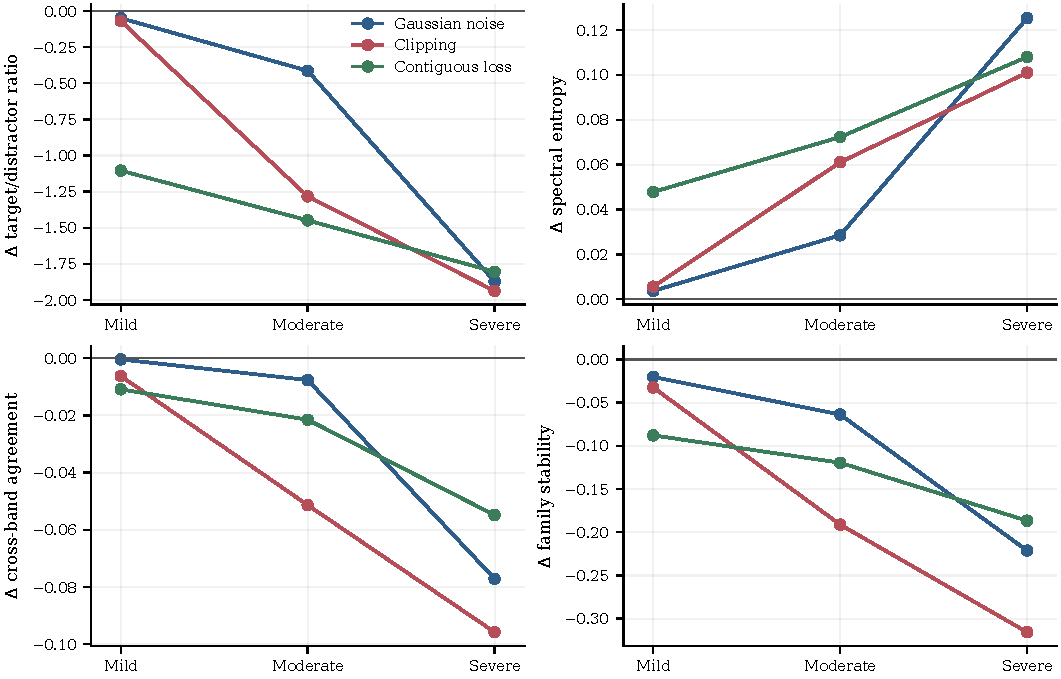
\includegraphics[width=0.92\textwidth]{representation_degradation.pdf}
\caption{Paired representation changes under controlled degradation. Noise, clipping, and contiguous loss share decreasing target dominance and consistency with increasing entropy, while their severity profiles remain mechanism-specific.}
\label{fig:degradation}
\end{figure*}

A descriptive principal-component analysis of paired T/D, entropy, cross-band agreement, and family-stability changes found that the first component explained 49.61\% of variation, with loadings $-0.547$, $+0.605$, $-0.417$, and $-0.402$, respectively. After standardization by clean non-failure variability, the feature-direction cosine between natural representation failures and severe degradation was 0.789 for noise, 0.924 for clipping, and 0.786 for sample loss. These similarities do not identify the physical cause of natural errors; they indicate a shared representation-level signature.

Positive attenuation after standardization caused no measurable change at any severity. Linear filtering, rectification, spectral ranking, and peak timing are invariant or equivariant to positive scalar gain in the absence of a fixed noise or quantization floor. Attenuation alone therefore does not simulate weak sensor coupling after z-score normalization.

\subsection{Waveform repair versus task fidelity}
Conventional recovery did not reliably restore representation. Under 0-dB noise, band-limiting recovered 53.7\% of waveform RMSE but changed HeartV6 MAE only from 4.086 to 4.036~BPM. Severe clipping interpolation worsened MAE from 4.491 to 7.890~BPM and material-failure rate from 14.95\% to 31.90\%. With 30\% contiguous loss, zero fill yielded 3.272~BPM MAE, compared with 3.340 for linear interpolation and 3.349 for PCHIP.

\begin{figure*}[t]
\centering
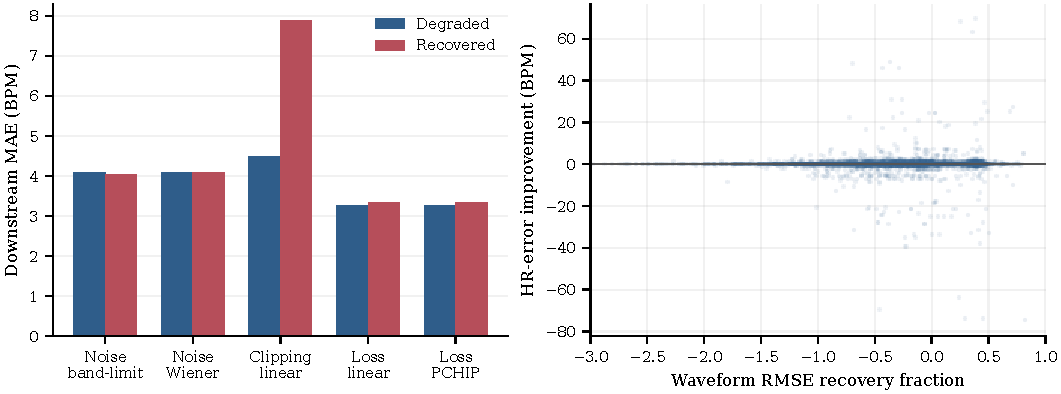
\includegraphics[width=0.94\textwidth]{reconstruction_task_mismatch.pdf}
\caption{Conventional reconstruction and downstream fidelity. Severe-condition MAE changes were marginal for noise filtering and adverse for clipping or missing-sample interpolation (left). Across paired cases, waveform RMSE recovery was weakly related to HR-error improvement (right; display truncated to the central waveform-recovery range for readability).}
\label{fig:reconstruction}
\end{figure*}

Across evaluated triplets, waveform RMSE recovery had Spearman association $\rho=0.067$ with final-HR error improvement and $\rho=0.173$ with T/D improvement. Severe clipping interpolation recovered 266 existing failures but induced 1,793 new failures. Severe sample-loss linear interpolation recovered 258 but induced 374. Generic smoothness or waveform similarity therefore did not constitute a reliable cardiac-information objective for this estimator.

\section{Discussion}
\subsection{What the estimator uses}
The controlled modulation experiment establishes that rectification and related nonlinear operations can expose low-frequency periodicity encoded in higher-frequency components. Real successful windows likewise contain target-aligned evidence across several mechanical bands, sometimes with higher bands preferring cardiac harmonics. This qualitative consistency supports envelope-based representation as an engineering mechanism, not a claim that real BCG follows the synthetic amplitude-modulation equation.

HeartV6 performance depends on structured evidence distributed across target dominance, spectral concentration, agreement among bands, and harmonic-family organization. No single diagnostic is sufficient: cross-band agreement can be high when all bands agree on the wrong family, and score margin is not monotonic with error. The multifeature degradation axis and unresolved failures both argue against reducing signal quality to one amplitude or confidence statistic.

\subsection{Representation failure and scoring}
Representation weakness was the largest resolved failure category. The scorer nonetheless shapes how weak evidence becomes an estimate. Its implicit low-frequency prior can cause lower-boundary locking, yet removing the prior produces many double-rate selections. This trade-off explains why scorer tuning was not pursued further: the primary deficiency is often the evidence supplied to the scorer, and a local scoring change can exchange one error family for another.

\subsection{Waveform fidelity is not task fidelity}
The reconstruction study provides the central negative result. A filter can reduce sample-wise waveform error without restoring the low-frequency, cross-band, or harmonic structure used by HeartV6. Conversely, interpolation may create a smooth waveform while erasing extrema or inventing periodic content. This does not imply that waveform reconstruction is universally ineffective; it shows misalignment for the evaluated conventional methods, disturbances, recordings, representation, and downstream estimator.

The appropriate design objective is therefore not merely visual or pointwise resemblance to a clean BCG. A recovery method should preserve cardiac information that remains stable across sensing conditions while controlling arbitrary waveform synthesis. This observation motivates task-aware representation learning, but the present study does not validate such a learned solution.

\section{Limitations}
All human recordings came from one individual. Repeated windows are dependent measurements, not independent biological samples, and no population-level or unseen-person generalization can be inferred. Exact continuous-source ancestry was verified, but higher recording-session relationships remain unknown. The ECG detector was audited algorithmically rather than against expert beat annotations.

Synthetic noise, clipping, and sample loss isolate sensing disturbances but do not reproduce the full dynamics of motion, posture, body coupling, mattress transfer, hardware saturation, or quantization. Post-normalization attenuation is a scale-invariance control, not a complete weak-coupling model. The modulation experiment demonstrates a DSP mechanism rather than physiological causation. Failure definitions use ECG information for research diagnosis and are not deployable BCG-only quality measures. HeartV6-specific representation findings may not generalize to other estimators. Conventional reconstruction conclusions apply only to the fixed methods tested here. Finally, the latent ECG--BCG framework below is proposed future work, not an implemented contribution.

\section{Future Work}
\subsection{Shared latent cardiac process}
ECG and BCG should not be treated as though one waveform were simply a filtered copy of the other. A more useful hypothesis is that both observe a shared latent cardiac process $z(t)$ through different physical pathways. If heartbeat times are $t_1,\ldots,t_N$, with $RR_i=t_{i+1}-t_i$, the process may include mean rate, beat-timing variability, respiratory modulation, and timing perturbations. Simplified observations could be
\begin{align}
e(t)&=\sum_i E(t-t_i;\theta_E)+\eta_E(t),\\
b_{\mathrm{card}}(t)&=\sum_i B(t-t_i-\tau_B;\theta_B),\\
h_{\mathrm{tot}}&=h_{\mathrm{body}}*h_{\mathrm{support}}*h_{\mathrm{sensor}},\\
y_{\mathrm{BCG}}(t)&=(h_{\mathrm{tot}}*b_{\mathrm{card}})(t)\notag\\
&\quad+r(t)+m(t)+\eta_B(t),
\end{align}
where $E$ and $B$ are electrical and mechanical beat templates, $h$ terms are transfer responses, $r$ is respiration, $m$ is motion, and $\eta$ terms are noise. Resonance, damping, mechanical delay, coupling, harmonic structure, and respiratory modulation would be controllable. Such a simulator would support hypothesis testing, not substitute for physiological validation.

\begin{figure}[t]
\centering
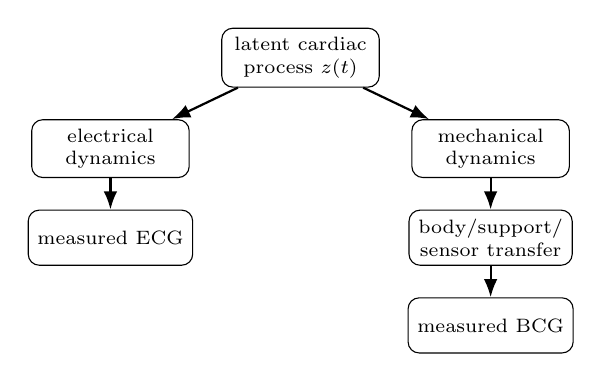
\begin{tikzpicture}[>=Latex,node distance=4mm and 4mm,
box/.style={draw,rounded corners,align=center,font=\scriptsize,minimum width=20mm,minimum height=7mm},arrow/.style={->,thick}]
\node[box] (z) {latent cardiac\\process $z(t)$};
\node[box,below left=of z] (el) {electrical\\dynamics};
\node[box,below right=of z] (mech) {mechanical\\dynamics};
\node[box,below=of el] (ecg) {measured ECG};
\node[box,below=of mech] (transfer) {body/support/\\sensor transfer};
\node[box,below=of transfer] (bcg) {measured BCG};
\draw[arrow] (z)--(el); \draw[arrow] (z)--(mech); \draw[arrow] (el)--(ecg); \draw[arrow] (mech)--(transfer); \draw[arrow] (transfer)--(bcg);
\end{tikzpicture}
\caption{Proposed future generative view: ECG and BCG are distinct observations of a shared latent cardiac process, with BCG additionally shaped by mechanical transfer and sensing conditions.}
\label{fig:latent}
\end{figure}

The existing modulation model is one deliberately simplified mechanism for asking when low-frequency periodicity is encoded in higher mechanical frequencies. A broader paired simulator could test when the fundamental becomes weaker than harmonics, which resonances preserve timing, how coupling changes multi-band evidence, and which parameter combinations reproduce observed failure signatures.

\subsection{Cross-modal representation learning}
Future learning should test whether a BCG encoder preserves cardiac information shared with an ECG-derived teacher, rather than optimizing only sample-wise BCG reconstruction. Candidate ECG supervision includes beat timing, cardiac phase, instantaneous rate, periodic time--frequency structure, or a learned embedding. Representation alignment must be paired with identity and bounded-residual constraints to prevent arbitrary signal synthesis.

The smallest fair next experiment would reuse the existing identity-initialized one-dimensional residual filter with one fixed architecture and verified continuous-source-held-out evaluation. A waveform-only objective would be compared with a prespecified representation-aware objective targeting spectral concentration, cross-band consistency, and harmonic-family stability. Clean identity controls, recovered and induced failures, and source-level heterogeneity should be reported. This is a research hypothesis; improved performance is not assumed.

\section{Conclusion}
Across repeated recordings from one individual, accurate BCG heart-rate estimation depended on preserving cardiac structure distributed across rectified spectra, mechanical bands, and harmonic families. Controlled degradation weakened this structure along a partly shared representation-quality axis, and representation weakness was the largest resolved failure mechanism. Conventional filtering and interpolation did not reliably restore the lost information: waveform reconstruction could improve signal similarity with negligible cardiac benefit or could create new estimation failures. For the evaluated pipeline, waveform fidelity and downstream cardiac-information fidelity are therefore distinct objectives. The resulting research direction is to preserve task-relevant cardiac representation explicitly, while validating any future learned method with strict continuous-source grouping and without interpreting synthetic diversity as human generalization.

\section*{Reproducibility Statement}
The project includes deterministic provenance validation, fixed perturbation configurations, estimator instrumentation, paired window/source summaries, and scripts for aggregate figure generation. Publication figures contain aggregate results only; raw BCG/ECG recordings and per-window personal-data-derived outputs are excluded. Historical results remain available for traceability under the corrected single-person interpretation.

\bibliographystyle{plainnat}
\bibliography{references}
\end{document}
